%%*************************************************************************
%% Legal Notice:
%% This code is offered as-is without any warranty either expressed or
%% implied; without even the implied warranty of MERCHANTABILITY or
%% FITNESS FOR A PARTICULAR PURPOSE! 
%% User assumes all risk.
%% In no event shall IEEE or any contributor to this code be liable for
%% any damages or losses, including, but not limited to, incidental,
%% consequential, or any other damages, resulting from the use or misuse
%% of any information contained here.
%%
%% All comments are the opinions of their respective authors and are not
%% necessarily endorsed by the IEEE.
%%
%% This work is distributed under the LaTeX Project Public License (LPPL)
%% ( http://www.latex-project.org/ ) version 1.3, and may be freely used,
%% distributed and modified. A copy of the LPPL, version 1.3, is included
%% in the base LaTeX documentation of all distributions of LaTeX released
%% 2003/12/01 or later.
%% Retain all contribution notices and credits.
%% ** Modified files should be clearly indicated as such, including  **
%% ** renaming them and changing author support contact information. **
%%
%% File list of work: IEEEtran.cls, IEEEtran_HOWTO.pdf, bare_adv.tex,
%%                    bare_conf.tex, bare_jrnl.tex, bare_jrnl_compsoc.tex
%%*************************************************************************

% *** Authors should verify (and, if needed, correct) their LaTeX system  ***
% *** with the testflow diagnostic prior to trusting their LaTeX platform ***
% *** with production work. IEEE's font choices can trigger bugs that do  ***
% *** not appear when using other class files.                            ***
% The testflow support page is at:
% http://www.michaelshell.org/tex/testflow/



% Note that the a4paper option is mainly intended so that authors in
% countries using A4 can easily print to A4 and see how their papers will
% look in print - the typesetting of the document will not typically be
% affected with changes in paper size (but the bottom and side margins will).
% Use the testflow package mentioned above to verify correct handling of
% both paper sizes by the user's LaTeX system.
%
% Also note that the "draftcls" or "draftclsnofoot", not "draft", option
% should be used if it is desired that the figures are to be displayed in
% draft mode.
%
\documentclass[conference]{IEEEtran}
% Add the compsoc option for Computer Society conferences.
%
% If IEEEtran.cls has not been installed into the LaTeX system files,
% manually specify the path to it like:
% \documentclass[conference]{../sty/IEEEtran}





% Some very useful LaTeX packages include:
% (uncomment the ones you want to load)


% *** MISC UTILITY PACKAGES ***
%
%\usepackage{ifpdf}
% Heiko Oberdiek's ifpdf.sty is very useful if you need conditional
% compilation based on whether the output is pdf or dvi.
% usage:
% \ifpdf
%   % pdf code
% \else
%   % dvi code
% \fi
% The latest version of ifpdf.sty can be obtained from:
% http://www.ctan.org/tex-archive/macros/latex/contrib/oberdiek/
% Also, note that IEEEtran.cls V1.7 and later provides a builtin
% \ifCLASSINFOpdf conditional that works the same way.
% When switching from latex to pdflatex and vice-versa, the compiler may
% have to be run twice to clear warning/error messages.
\usepackage[utf8x]{inputenc}





% *** CITATION PACKAGES ***
%
%\usepackage{cite}
% cite.sty was written by Donald Arseneau
% V1.6 and later of IEEEtran pre-defines the format of the cite.sty package
% \cite{} output to follow that of IEEE. Loading the cite package will
% result in citation numbers being automatically sorted and properly
% "compressed/ranged". e.g., [1], [9], [2], [7], [5], [6] without using
% cite.sty will become [1], [2], [5]--[7], [9] using cite.sty. cite.sty's
% \cite will automatically add leading space, if needed. Use cite.sty's
% noadjust option (cite.sty V3.8 and later) if you want to turn this off.
% cite.sty is already installed on most LaTeX systems. Be sure and use
% version 4.0 (2003-05-27) and later if using hyperref.sty. cite.sty does
% not currently provide for hyperlinked citations.
% The latest version can be obtained at:
% http://www.ctan.org/tex-archive/macros/latex/contrib/cite/
% The documentation is contained in the cite.sty file itself.






% *** GRAPHICS RELATED PACKAGES ***
%
\ifCLASSINFOpdf
	\usepackage[pdftex]{graphicx}
  % declare the path(s) where your graphic files are
  % \graphicspath{{../pdf/}{../jpeg/}}
  % and their extensions so you won't have to specify these with
  % every instance of \includegraphics
  % \DeclareGraphicsExtensions{.pdf,.jpeg,.png}
\else
  % or other class option (dvipsone, dvipdf, if not using dvips). graphicx
  % will default to the driver specified in the system graphics.cfg if no
  % driver is specified.
  % \usepackage[dvips]{graphicx}
  % declare the path(s) where your graphic files are
  % \graphicspath{{../eps/}}
  % and their extensions so you won't have to specify these with
  % every instance of \includegraphics
  % \DeclareGraphicsExtensions{.eps}
\fi
% graphicx was written by David Carlisle and Sebastian Rahtz. It is
% required if you want graphics, photos, etc. graphicx.sty is already
% installed on most LaTeX systems. The latest version and documentation can
% be obtained at: 
% http://www.ctan.org/tex-archive/macros/latex/required/graphics/
% Another good source of documentation is "Using Imported Graphics in
% LaTeX2e" by Keith Reckdahl which can be found as epslatex.ps or
% epslatex.pdf at: http://www.ctan.org/tex-archive/info/
%
% latex, and pdflatex in dvi mode, support graphics in encapsulated
% postscript (.eps) format. pdflatex in pdf mode supports graphics
% in .pdf, .jpeg, .png and .mps (metapost) formats. Users should ensure
% that all non-photo figures use a vector format (.eps, .pdf, .mps) and
% not a bitmapped formats (.jpeg, .png). IEEE frowns on bitmapped formats
% which can result in "jaggedy"/blurry rendering of lines and letters as
% well as large increases in file sizes.
%
% You can find documentation about the pdfTeX application at:
% http://www.tug.org/applications/pdftex





% *** MATH PACKAGES ***
%
\usepackage[cmex10]{amsmath}
% A popular package from the American Mathematical Society that provides
% many useful and powerful commands for dealing with mathematics. If using
% it, be sure to load this package with the cmex10 option to ensure that
% only type 1 fonts will utilized at all point sizes. Without this option,
% it is possible that some math symbols, particularly those within
% footnotes, will be rendered in bitmap form which will result in a
% document that can not be IEEE Xplore compliant!
%
% Also, note that the amsmath package sets \interdisplaylinepenalty to 10000
% thus preventing page breaks from occurring within multiline equations. Use:
%\interdisplaylinepenalty=2500
% after loading amsmath to restore such page breaks as IEEEtran.cls normally
% does. amsmath.sty is already installed on most LaTeX systems. The latest
% version and documentation can be obtained at:
% http://www.ctan.org/tex-archive/macros/latex/required/amslatex/math/





% *** SPECIALIZED LIST PACKAGES ***
%
%\usepackage{algorithmic}
% algorithmic.sty was written by Peter Williams and Rogerio Brito.
% This package provides an algorithmic environment fo describing algorithms.
% You can use the algorithmic environment in-text or within a figure
% environment to provide for a floating algorithm. Do NOT use the algorithm
% floating environment provided by algorithm.sty (by the same authors) or
% algorithm2e.sty (by Christophe Fiorio) as IEEE does not use dedicated
% algorithm float types and packages that provide these will not provide
% correct IEEE style captions. The latest version and documentation of
% algorithmic.sty can be obtained at:
% http://www.ctan.org/tex-archive/macros/latex/contrib/algorithms/
% There is also a support site at:
% http://algorithms.berlios.de/index.html
% Also of interest may be the (relatively newer and more customizable)
% algorithmicx.sty package by Szasz Janos:
% http://www.ctan.org/tex-archive/macros/latex/contrib/algorithmicx/




% *** ALIGNMENT PACKAGES ***
%
%\usepackage{array}
% Frank Mittelbach's and David Carlisle's array.sty patches and improves
% the standard LaTeX2e array and tabular environments to provide better
% appearance and additional user controls. As the default LaTeX2e table
% generation code is lacking to the point of almost being broken with
% respect to the quality of the end results, all users are strongly
% advised to use an enhanced (at the very least that provided by array.sty)
% set of table tools. array.sty is already installed on most systems. The
% latest version and documentation can be obtained at:
% http://www.ctan.org/tex-archive/macros/latex/required/tools/


%\usepackage{mdwmath}
%\usepackage{mdwtab}
% Also highly recommended is Mark Wooding's extremely powerful MDW tools,
% especially mdwmath.sty and mdwtab.sty which are used to format equations
% and tables, respectively. The MDWtools set is already installed on most
% LaTeX systems. The lastest version and documentation is available at:
% http://www.ctan.org/tex-archive/macros/latex/contrib/mdwtools/


% IEEEtran contains the IEEEeqnarray family of commands that can be used to
% generate multiline equations as well as matrices, tables, etc., of high
% quality.


%\usepackage{eqparbox}
% Also of notable interest is Scott Pakin's eqparbox package for creating
% (automatically sized) equal width boxes - aka "natural width parboxes".
% Available at:
% http://www.ctan.org/tex-archive/macros/latex/contrib/eqparbox/





% *** SUBFIGURE PACKAGES ***
%\usepackage[tight,footnotesize]{subfigure}
% subfigure.sty was written by Steven Douglas Cochran. This package makes it
% easy to put subfigures in your figures. e.g., "Figure 1a and 1b". For IEEE
% work, it is a good idea to load it with the tight package option to reduce
% the amount of white space around the subfigures. subfigure.sty is already
% installed on most LaTeX systems. The latest version and documentation can
% be obtained at:
% http://www.ctan.org/tex-archive/obsolete/macros/latex/contrib/subfigure/
% subfigure.sty has been superceeded by subfig.sty.



%\usepackage[caption=false]{caption}
%\usepackage[font=footnotesize]{subfig}
% subfig.sty, also written by Steven Douglas Cochran, is the modern
% replacement for subfigure.sty. However, subfig.sty requires and
% automatically loads Axel Sommerfeldt's caption.sty which will override
% IEEEtran.cls handling of captions and this will result in nonIEEE style
% figure/table captions. To prevent this problem, be sure and preload
% caption.sty with its "caption=false" package option. This is will preserve
% IEEEtran.cls handing of captions. Version 1.3 (2005/06/28) and later 
% (recommended due to many improvements over 1.2) of subfig.sty supports
% the caption=false option directly:
%\usepackage[caption=false,font=footnotesize]{subfig}
%
% The latest version and documentation can be obtained at:
% http://www.ctan.org/tex-archive/macros/latex/contrib/subfig/
% The latest version and documentation of caption.sty can be obtained at:
% http://www.ctan.org/tex-archive/macros/latex/contrib/caption/




% *** FLOAT PACKAGES ***
%
%\usepackage{fixltx2e}
% fixltx2e, the successor to the earlier fix2col.sty, was written by
% Frank Mittelbach and David Carlisle. This package corrects a few problems
% in the LaTeX2e kernel, the most notable of which is that in current
% LaTeX2e releases, the ordering of single and double column floats is not
% guaranteed to be preserved. Thus, an unpatched LaTeX2e can allow a
% single column figure to be placed prior to an earlier double column
% figure. The latest version and documentation can be found at:
% http://www.ctan.org/tex-archive/macros/latex/base/



%\usepackage{stfloats}
% stfloats.sty was written by Sigitas Tolusis. This package gives LaTeX2e
% the ability to do double column floats at the bottom of the page as well
% as the top. (e.g., "\begin{figure*}[!b]" is not normally possible in
% LaTeX2e). It also provides a command:
%\fnbelowfloat
% to enable the placement of footnotes below bottom floats (the standard
% LaTeX2e kernel puts them above bottom floats). This is an invasive package
% which rewrites many portions of the LaTeX2e float routines. It may not work
% with other packages that modify the LaTeX2e float routines. The latest
% version and documentation can be obtained at:
% http://www.ctan.org/tex-archive/macros/latex/contrib/sttools/
% Documentation is contained in the stfloats.sty comments as well as in the
% presfull.pdf file. Do not use the stfloats baselinefloat ability as IEEE
% does not allow \baselineskip to stretch. Authors submitting work to the
% IEEE should note that IEEE rarely uses double column equations and
% that authors should try to avoid such use. Do not be tempted to use the
% cuted.sty or midfloat.sty packages (also by Sigitas Tolusis) as IEEE does
% not format its papers in such ways.





% *** PDF, URL AND HYPERLINK PACKAGES ***
%
%\usepackage{url}
% url.sty was written by Donald Arseneau. It provides better support for
% handling and breaking URLs. url.sty is already installed on most LaTeX
% systems. The latest version can be obtained at:
% http://www.ctan.org/tex-archive/macros/latex/contrib/misc/
% Read the url.sty source comments for usage information. Basically,
% \url{my_url_here}.
\usepackage{hyperref}





% *** Do not adjust lengths that control margins, column widths, etc. ***
% *** Do not use packages that alter fonts (such as pslatex).         ***
% There should be no need to do such things with IEEEtran.cls V1.6 and later.
% (Unless specifically asked to do so by the journal or conference you plan
% to submit to, of course. )


% correct bad hyphenation here
\hyphenation{op-tical net-works semi-conduc-tor}


\begin{document}
%
% paper title
% can use linebreaks \\ within to get better formatting as desired
\title{A Scalable Algorithm for Similar Image Detection}


% author names and affiliations
% use a multiple column layout for up to three different
% affiliations


% conference papers do not typically use \thanks and this command
% is locked out in conference mode. If really needed, such as for
% the acknowledgment of grants, issue a \IEEEoverridecommandlockouts
% after \documentclass

% for over three affiliations, or if they all won't fit within the width
% of the page, use this alternative format:
% 

\author{
\IEEEauthorblockN{Andrei-Bogdan Pârvu}
\IEEEauthorblockA{Computer Science and Engineering Department\\
Faculty of Automatic Control and Computers \\
POLITEHNICA University of Bucharest\\
Email: andrei.parvu@cti.pub.ro}
\and
\IEEEauthorblockN{Nicolae Țăpuș}
\IEEEauthorblockA{Computer Science and Engineering Department\\
Faculty Automatic Control and Computers \\
POLITEHNICA University of Bucharest\\
Email: nicolae.tapus@cs.pub.ro}\\
\IEEEauthorblockN{Virgil Palanciuc}
\IEEEauthorblockA{Adobe Systems Romania\\
Email: virgilp@adobe.com}
\and
\IEEEauthorblockN{Ștefan-Teodor Crăciun}
\IEEEauthorblockA{Adobe Systems Romania\\
Email: scraciun@adobe.com} 
}


% use for special paper notices
%\IEEEspecialpapernotice{(Invited Paper)}


% make the title area
\maketitle


\begin{abstract}
%\boldmath
In this paper, we propose an algorithm for detecting similar images in a large scale dataset. After considering various methods as invisible watermarking and image feature detection, we developed a method based on the $Harris\ corner\ detection$ and the $Scale\ Invariant\ Feature\ Transform$ keypoints and descriptors for analyzing the properties of an image.\\
Our goal is that the proposed algorithm be resilient to watermarked, scaled or cropped images, and provide a fast running time for our large dataset.\\
In order to be able to handle a large amount of images and associated data, we have decided to maintain the descriptors of the images in a set of KD-tree structures for fast querying. This allows an initial filtering of the data set, reducing the number of images which should be analyzed. Thus, we will use two search algorithms, one of which has a lower time complexity, but has a lower accuracy when providing the results, and a second one, which performed a more in-depth analysis of the images.\\
\end{abstract}
% IEEEtran.cls defaults to using nonbold math in the Abstract.
% This preserves the distinction between vectors and scalars. However,
% if the conference you are submitting to favors bold math in the abstract,
% then you can use LaTeX's standard command \boldmath at the very start
% of the abstract to achieve this. Many IEEE journals/conferences frown on
% math in the abstract anyway.

% no keywords




% For peer review papers, you can put extra information on the cover
% page as needed:
% \ifCLASSOPTIONpeerreview
% \begin{center} \bfseries EDICS Category: 3-BBND \end{center}
% \fi
%
% For peerreview papers, this IEEEtran command inserts a page break and
% creates the second title. It will be ignored for other modes.
\IEEEpeerreviewmaketitle



\section{Introduction}
Image processing has been a very important research domain the last years, the ever increasing number of images present on the Internet becoming more and more challenging to index, store and analyze.\\
Copyright infringement and image detection have also been big issues which have been discussed and studied for a long time, major users in the photography industry wanting to know at all times when someone is using or modifying one of their photos.\\
The problem discussed in this paper is considered a very difficult one, because the algorithm needs to be at the same time accurate, fast and scalable. \\

Our goal was to design a scalable algorithm which can index information about a large set of images, and perform queries of finding a highly similar image with a given input one. \\
The algorithm should be focused on copyright detection, so it should be able to determine if the input image is one of the images in the dataset, with one or several of the following transformations applied:
\begin{itemize}
	\item watermarks
	\item scaling
	\item cropping
	\item various filters
\end{itemize}

As said above, the granularity of the algorithm should be set so that it should be able to distinguish between two lightly similar images (e.g. two different pictures of the Eiffel Tower, made by two different persons) and two images, one of which is obtained from the other.\\

The speed and scalability of the algorithm are also major factors which should be seriously taken into consideration. It should be able to handle a large number of queries and provide a small response-time per query. Of course, there is a close connection between the running time of the algorithm and its precision, connection which should be closely analyzed in order to create a balance between the two.

\hfill June 2014

\section{Previous Work}

During the first phase of our research, we collected about $4500$ images from the Internet (various stock photography sites), which we classified into similarity sets. The images comprising a similarity set should be roughly the same, with differences only in size, rotation and various applied
watermarks.\\
We searched for a simple, fast to implement method of doing this, before diving into something more elaborate.
We decided to compute a 64-bit hash for each image, and then use the Hamming distance between two hashes to measure the degree
to similarity between the images. The three types of hashes that we computed and analyzed are:
\begin{itemize}
  \item average hash: reduce the image to a $8\times8$ grayscale; each bit in the 64-bit hash will be either 0, if the corresponding
  pixel value is lower than the average of all pixels' values, or, in the other case, 1.
  \item perceptive hash: similar with the average hash, but instead of comparing the pixel values it used the Discrete Cosine Transform
  for the image.
  \item difference hash: reduce the image to a $9\times8$ grayscale; compute the difference between each horizontally adjacent pixels and
  set the corresponding bit in the hash to 1, if the difference is smaller than 0, or to 1 otherwise.
\end{itemize}

For checking if a given image is present in our set of already stored images, we just compute one of its hashes (average, perceptive
or difference) and compare it with the already determined hashes. Experimentally, we have determined that two images with a Hamming
distance of their corresponding hashes less than 19 are similar.\\
Of course, the search requires a running time of $O(n)$, where $n$ is the number of stored images, which is not good enough for a large
size of the image set. A further optimization that can reduce the running time of the search is using a locality sensitive hash, but this
exceeds the desired simplicity of our initial method.\\
It is worth mentioning that out of the three possible hashes, the best results were obtained with the difference hash, because of its
small computation time and its accuracy.


\section{Related Algorithms}

There are a lot of algorithms which focus on image similarity and key feature detection, and after studying several ones, we decided on focusing on two main ones, the $Harris\ corner\ detector$ and the $Scale\ Invariant$ $Feature\ Transform$. Our choice was determined on the fact we wanted to be able to control the sensitivity of the matches, but also to efficiently distribute the algorithm on several machines for a large input set. \\


\subsection{Harris Corner Detection}

The main idea of the $Harris\ corner\ detector$ algorithm is that, given an input image, the most predominant features that a human eye recognizes and memorizes are corners. A corner is considered to be an intersection of two edges, so, selecting a small area around the point and shifting it should result in a large variation in the intensity of the pixels in that area. \\
Therefore, each area in an image can be classified in three categories:
\begin{itemize}
	\item flat, in which intensities do not vary in either direction
	\item edge, in which intensities don't vary in the direction of the edge
	\item corner, in which intensities vary in all directions
\end{itemize}

In order to determine in which category a certain area with a size of $(w, h)$ belongs to, we will compute the variation of intensity: $E(w, h) = \sum_{x, y} w(x, y) * [I(x + w, y + h) - I(x, y)]^2$, where $w$ is a window function, which assigns weights to pixels, and $I$ is the intensity of a certain pixel of the grayscale image.\\
In order to determine the corner areas, we have to maximize the function $\sum_{x, y}[I(x + w, y + v) - I(x, y)]^2$, which using $Taylor$ expansion and representing in a matrix form can be written as
$E(w, h) \approx
\begin{bmatrix}
w & h
\end{bmatrix} * 
\left(\sum_{x, y}
\begin{bmatrix}
I_x^2 & I_xI_y\\
I_xI_y & I_y^2
\end{bmatrix}
\right) *
\begin{bmatrix}
w \\
h
\end{bmatrix}$, and, furthermore, using a substitution
$E(w, h) \approx
\begin{bmatrix}
w & h
\end{bmatrix} * 
M *
\begin{bmatrix}
w \\
h
\end{bmatrix}$.\\
Using this equation, the score of a certain area is computed as $R = det(M) - k * (trace(M))^2$. A higher score of $R$ denotes a higher probability of the area being a corner.

\subsection{Scale Invariant Feature Transform}
\subsubsection{Keypoint localization}
Although the $Harris\ corner\ detection$ algorithm presented in the previous section is immune to rotation transformations of an image, it does not perform well if the image is scaled, because a high intensity change in an area of size $(w, h)$ of an image might vary if the dimensions of the image change, but the size of the area remains the same.\\
Thus, D. Lowe, in 2004, presented a new algorithm for extracting keypoints and computing their descriptors, named $Scale\ Invariant\ Feature\ Transform$.\\
At first, a Gaussian distribution is applied on the analyzed image, which depending of the standard deviation, $\sigma$, blurs the image with a certain amount: $G(x, y) = \frac{1}{2 * \pi * \sigma^2} * e^{-\frac{x^2 + y^2}{2 * \sigma^2}}$.\\
Then, the Laplacian of the image is computed, in order to highlight the regions of rapid intensity changes: $L(x, y) = \frac{\delta^2 I}{\delta x^2} + \frac{\delta^2 I}{\delta y^2}$. Combined with the previous Gaussian filter, we obtain the so called Laplacian of Gaussian: $LoG(x, y) = -\frac{1}{\pi * \sigma^4} * \left(1 - \frac{x^2 + y^2}{2 * \sigma^2}\right) * e^{-\frac{x^2 + y^2}{2 * \sigma^2}}$.\\
Because the $LoG$ has a high computational cost, it is approximated with a Difference of Gaussians, which is a difference of two Gaussians with two different $\sigma$ deviations, representing two different scaled images. The local extrema of the computed $DoG$ are considered potential keypoints.
\subsubsection{Computing the Descriptors}
Once we have the keypoints, the corresponding descriptors are computed by taking a $16\times16$ neighborhood around the keypoint, and creating a $8$ bin histogram for each sub-block of $4\times4$ size of the initial neighborhood. Thus, a keypoint descriptor will contain $128$ values.


\section{The Image Similarity Algorithm}
\label{section:algorithm}

The algorithm we developed is composed out of two parts:
\begin{itemize}
	\item the analysis of a pair of images, in which we try to determine the degree of similarity between two images
	\item the retrieval of a small subset of likely candidates of similarity from a large image database
\end{itemize}

\subsection{Analysis of a pair of images}
In order to analyze a pair of images, we used the SIFT descriptors determined in the previous section. The two sets of descriptors are compared in order to obtain the best matches between pairs of keypoints. A distance is computed between each pair of keypoint descriptors, which is the Euclidian norm between the SIFT descriptors of the keypoints. Experimentally, we have concluded that a match between two keypoints has a high similarity if the Euclidian norm is less than $100$.\\
For a pair of images, we first find the set of SIFT components that are part of the Harris corner-mask and then compute the best matches between these keypoints. We have decided to use the corner-mask as a filtering mechanism for the SIFT keypoints in order to be able to potentially reduce the number of descriptors of a given image. We keep only the best $10$ matches, and compute the arithmetic mean between the distances of these matches; if this mean is smaller than $100$, the two images are considered similar. We shall name this algorithm the $pair\ similarity\ algorithm$ and the mean between the distances $image\ pair\ score$.\\
Figure~\ref{fig:compareImages} shows the corresponding matches between two images with two different watermarks, one of which is rotated $90^o$ clockwise.

\begin{figure}[ht!]
\centering
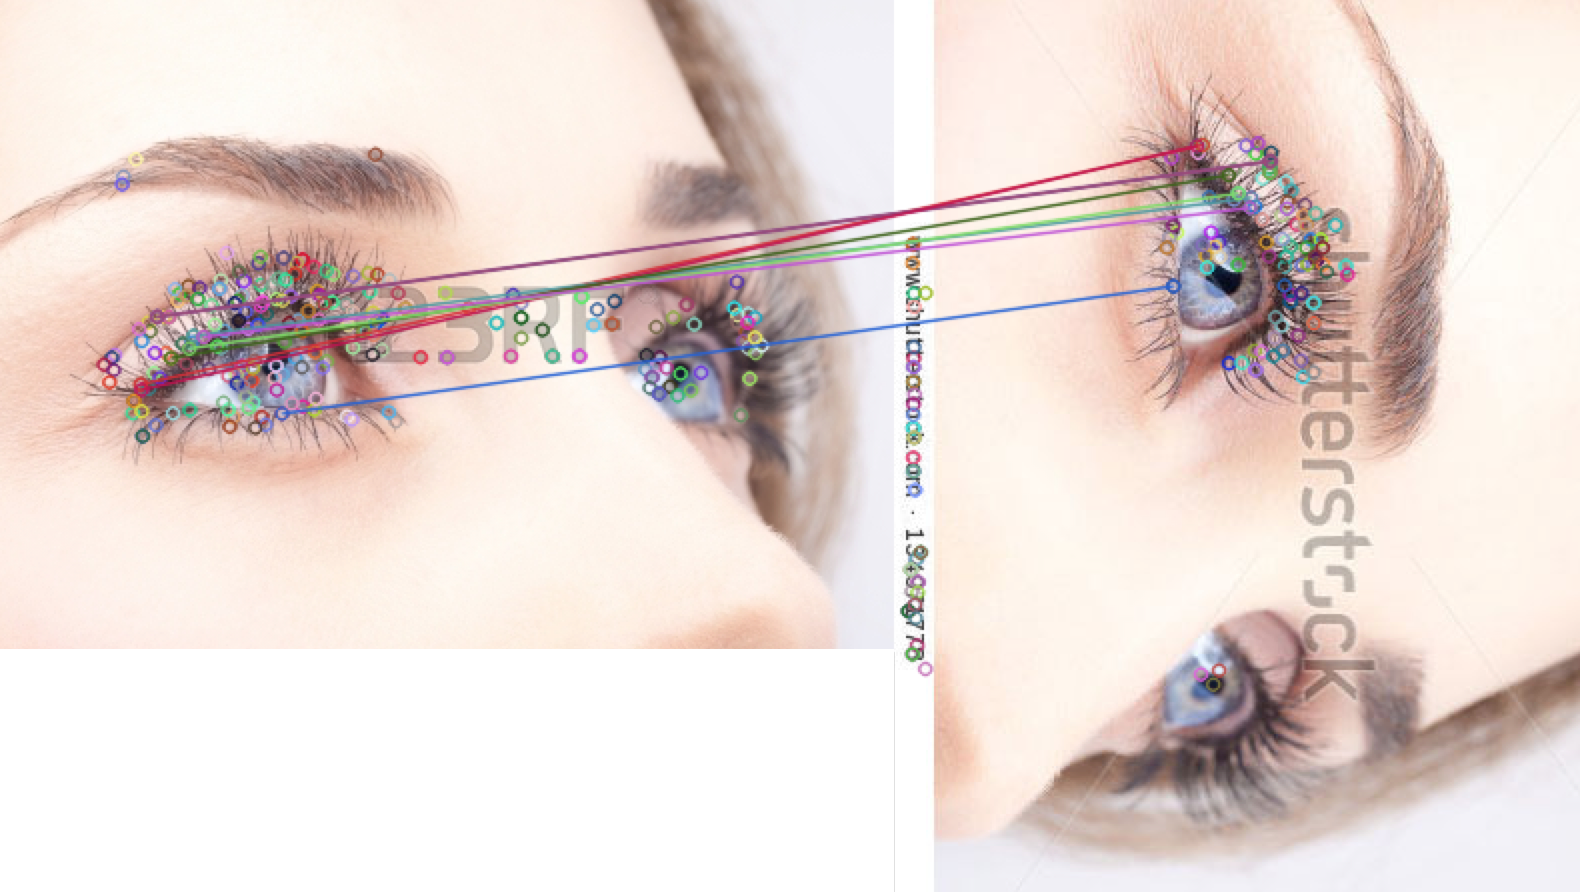
\includegraphics[width=.8\linewidth]{images/compare.png}
\caption{Comparison between two images}
\label{fig:compareImages}
\end{figure}

\subsection{Analysis of a set of images}

Suppose that we have a set of images, and we want to compare a test image with each image in the set and detect whether there exists a similar one. Of course, the first possibility is the brute force one: we iterate through all the images and apply the $pair\ similarity\ algorithm$ described in the previous section. Although this provides a correct result, it has a complexity of $O(number\_of\_images * image\_match\_time)$. We shall name this basic algorithm as the $linear\ algorithm$. Although this algorithm is very straightforward, its complexity is undesirable if the number of images becomes large (i.e. more than $500$). Moreover, most of the images in our set will likely have a big similarity distance with our searched image, so maybe we don't want to apply the full $pair\ similarity\ algorithm$.\\
Thus, we need to determine an efficient algorithm which can filter the initial set of images to a smaller set which contains the best possible candidates in terms of visual similarity.\\
The filtering algorithm is implemented as follows: we maintain a maximum number of $M$ descriptors for each image in the initial set and create $P$ KD-trees with the set of descriptors of the initial images. When a query for a test image arrives, we compute its descriptors and then perform a $K$ nearest-neighbor search on each of our KD-trees. Then, we select the top $T$ images returned from the nearest neighbor searches and perform the $linear\ algorithm$. We shall name this algorithm the $kdtree\ algorithm$.\\
Of course, the important factors in the $kdtree\ algorithm$ are:
\begin{itemize}
	\item the values of the numbers $M$, $T$ and $K$ from the above description
	\item the metric used in selecting the top $T$ images from the nearest-neighbor search
	\item the metric used in selecting the $M$ descriptors from the input images to form the KD-tree
	\item $N$, the number of images that form a KD-tree
	\item $P$, the number of KD-trees, which can be determined from the total number of images and $N$.
\end{itemize}

We propose three metrics in for selecting the filtered images from the KD-tree based on the nearest-neighbor search:
\begin{itemize}
	\item the images with the largest number of descriptors returned from the search
	\item the images with the smallest average of the distance of the found descriptors
	\item the images with the largest distance between its descriptors and the average of all found descriptors (from all the images)
\end{itemize}

The main problem when storing the descriptors in the KD-tree is in what form to have the images during the computation. We have three possibilities:
\begin{itemize}
	\item keep them in the original size
	\item resize all the images to a fixed dimension (eg. 400 × 300)
	\item resize all the images to a fixed width and scale the height
\end{itemize}

For the initial attempts, we have set the values of $M$, $T$ and $K$ to $40$, $10$ and $5$ and used the largest number of found descriptors as metric for selecting the filtered images from the KD-tree.\\

\subsection{Architecture of the application}
The basic structure of our application is maintaining a set of Image Servers, each containing a number of $R$ KD-trees to use for quering.
Thus, when a query arrives, we shall use a map-reduce technique: the query is distributed among the Image Servers, which compute the most similar images from their associated KD-tress and send the results back to a special entity called the Map Reducer. The Map Reducer combines these results, takes the best ones and sends them back to the quering entity.
 
\section{Data Set and Testing}

We have collected a set of $4500$ images from the Internet, which we have classified in about $1600$ similarity sets, each set being composed of up to five images. The images within a similarity set differ in size, having various watermarks and filters applied (these sets are known to be correct beforehand). We have inserted these images in a larger set of $100.000$ images taken from the Internet and performed a queries for each of the $4500$ images of the similarity sets, getting the top $10$ similar images. We want to observe:
\begin{itemize}
	\item if the algorithm finds the exact match, i.e. the image that has been queried with
	\item if the algorithm finds the other images which are part of the same similarity set
	\item the mean running time of a query
	\item how varying the metrics described above influences the results of the query
\end{itemize}

We evaluate the response to a query, by looking at the indices of the images from the current similarity set in the list of results returned by the query. Thus, the $index\ score$ for a certain query can be computed as the sum of these indices; the smaller the sum, the closer in the response list are the images we want to find. \\
For the set of $100.000$ images we use $P=20$ KD-trees, each KD-tree storing the descriptors for $N=5000$ images.\\
The results of this test can be seen in the following two tables. The first one describes, for similarity sets of size $3$, $4$ and $5$, and for the metrics described in \nameref{section:algorithm}, the average number of how many of these images are found in the list of $10$ returned images.\\

\begin{tabular} {c | c | c | c}
	& max nr descs & min avg & max dist to avg \\
	\hline
	3 & 2.47 & 2.37 & 2.52 \\
	\hline
	4 & 3.26 & 3.21 & 3.38 \\
	\hline
	5 & 3.98 & 3.63 & 4.14 \\
\end{tabular}

The second table shows the $index\ score$ (described above) for the same queries and metrics.\\

\begin{tabular} {c | c | c | c}
	& max nr descs & min avg & max dist to avg \\
	\hline
	3 & 8.32 & 9.29 & 7.84 \\
	\hline
	4 & 12.69 & 13.15 & 11.76 \\
	\hline
	5 & 18.35 & 21.36 & 17.10 \\
\end{tabular}

It can be observed that the third metric, the largest distance from the descriptors of an image to the average of all found descriptors, provides the best results.\\

We computed the descriptors for images resized to a fixed value (height $400$ and width $300$), and analyzed the same metrics and scores described above. The results can be seen in the tables below,
and they confirm that this image storing performs worse than the aspect-ratio one, so we have decided to continue using the first one.\\

\begin{tabular} {c | c | c | c}
	& max nr descs & min avg & max dist to avg \\
	\hline
	3 & 2.69 & 2.08 & 2.73 \\
	\hline
	4 & 3.55 & 2.60 & 3.62 \\
	\hline
	5 & 4.17 & 2.80 & 4.32 \\
\end{tabular}

\begin{tabular} {c | c | c | c}
	& max nr descs & min avg & max dist to avg \\
	\hline
	3 & 6.32 & 11.93 & 5.97 \\
	\hline
	4 & 10.37 & 18.46 & 9.84 \\
	\hline
	5 & 16.8 & 28.35 & 15.67 \\
\end{tabular}

As stated in \nameref{section:algorithm}, we decided to maintain multiple KD-trees in one Image Server in order to improve the quality of the heuristic search on one such KD-tree and reduce the total number of processes.\\
On the same set of $100.000$ images, we created $P=40$ Image Servers, with each server having $5000$ images and $R=2$ KD-trees (that means $N=2500$ images per KD-tree), so that we could compare the $correctness\ scores$ between this implementation and the one with $R=1$.\\
These are shown in the tables below:\\

\begin{tabular} {c | c | c | c}
	& max nr descs & min avg & max dist to avg \\
	\hline
	3 & 2.86 & 2.5 & 2.87 \\
	\hline
	4 & 3.83 & 3.35 & 3.85 \\
	\hline
	5 & 4.6 & 4.75 & 4.62 \\
\end{tabular}

\begin{tabular} {c | c | c | c}
	& max nr descs & min avg & max dist to avg \\
	\hline
	3 & 4.76 & 8.03 & 4.70 \\
	\hline
	4 & 7.96 & 11.92 & 7.82 \\
	\hline
	5 & 13.56 & 20.35 & 13.49 \\
\end{tabular}

It can be seen that the scores are comparable with the ones obtained from running the algorithm it the two cases shown in the previous subsections, so it can be confirmed that using multiple KD-trees of a fixed (and lesser size) is in our advantage when the overall dataset becomes larger, in order to avoid a large number of Image Servers.

Also, we have constructed a single KD-tree which contains the $4500$ images from the similarity set in order to test the three different metrics described in \nameref{section:algorithm} for selecting the filtered images.\\
We retained the $image\ pair\ score$ of the returned similar images, and evaluated these three metrics by computing the following $correctness\ scores$:
\begin{itemize}
	\item the mean between the $image\ pair\ scores$
	\item the sum of the differences between the $pair\ scores$ of two consecutive similar images in the returned list
	\item the maximum $image\ pair\ score$
\end{itemize}
The goal is to minimize each of these $correctness\ scores$.

The results of this test are shown in the next table:\\
\\
\begin{tabular} {c | c | c | c}
	& max nr descs & min avg & max dist to avg \\
	\hline
	mean & 661880 & 693745 & 647355 \\
	\hline
	sum of diff & 867877 & 1021543 & 856521 \\
	\hline
	max score & 1162618 & 1134470 & 1150899 \\
\end{tabular}

As it can be seen, the third metric, largest distance from the descriptors of an image to the average of all found descriptors, performs the best out of the three metrics.\\

Besides running the algorithm on our similarity sets, we also took some images from our $100.000$ set and used Google Image Search or TinEye to find replicas of those images on the Internet. Then we did a reverse search of those images with our algorithm to see if it finds the original images used in the query.\\
We had some interesting results, shown in Figure~\ref{fig:example1.1} and Figure~\ref{fig:example2.1}.\\

\begin{figure}[ht!]
\centering
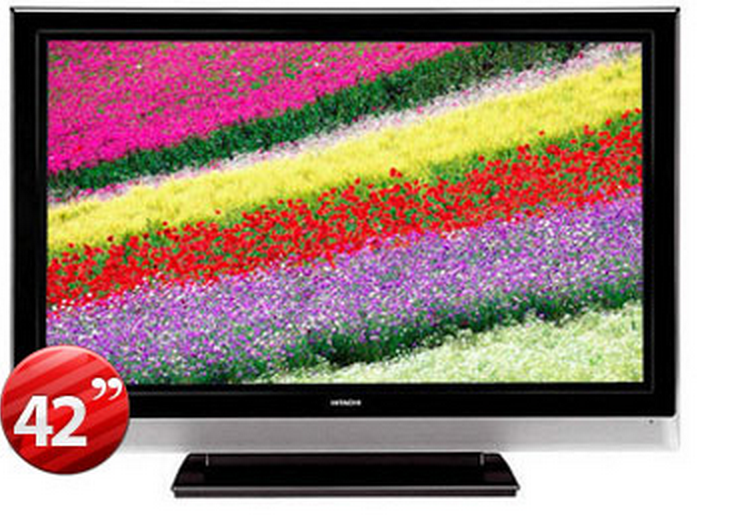
\includegraphics[width=.6\linewidth]{images/fieldSite.png}
\caption{Image from website}
\label{fig:example1.1}
\end{figure}

\begin{figure}[ht!]
\centering
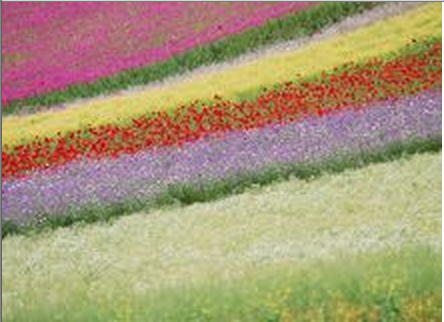
\includegraphics[width=.6\linewidth]{images/field.png}
\caption{Image from database}
\label{fig:example1.2}
\end{figure}


\begin{figure}[ht!]
\centering
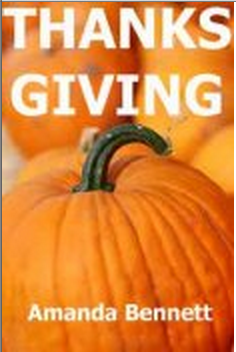
\includegraphics[width=.4\linewidth]{images/pumpkinSite.png}
\caption{Image from website}
\label{fig:example2.1}
\end{figure}

\begin{figure}[ht!]
\centering
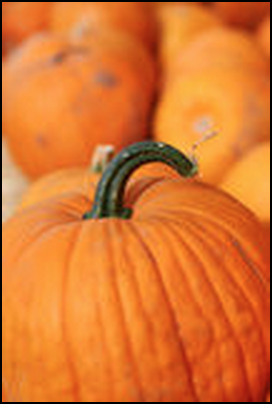
\includegraphics[width=.4\linewidth]{images/pumpkin.png}
\caption{Image from database}
\label{fig:example2.2}
\end{figure}

\subsection{Running Time}
We have tested our algorithm on a machine with 55GB of RAM, 16 quad-core processors with a frequency of 2.4GHz.
There are two different running times that we have been interested in: the first is the actual time that it takes for a query result to be computed - because of the heuristic search on the KD-tree with a limited depth, this will not vary very much when the KD-tree grows in size. For a number of $5000$ queries, the mean running time of a search on a KD-tree is $1.36$ seconds.\\
The second running time is the initialization of the KD-tree, which is divided into two steps: the computation of the descriptors for the images, and the construction of the actual KD-tree.\\
In Figure~\ref{fig:totalInit} we can see the total initialization time for a KD-tree, and the time needed only for the construction of the KD-tree data structure (presuming that the descriptors are already computed). \\
\begin{figure}[ht!]
\centering
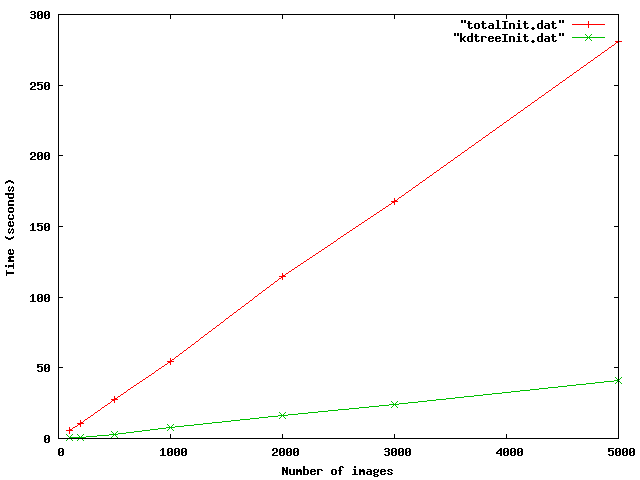
\includegraphics[width=.8\linewidth]{images/totalInit.png}
\caption{Initialization runtimes}
\label{fig:totalInit}
\end{figure}

\begin{tabular} {c | c | c}
	number of images & total init (seconds) & kdtree init (seconds) \\
	\hline
	100 & 5.34 & 0.48 \\
	200 & 10.53 & 0.99 \\
	500 & 27.71 & 3.17 \\
	1000 & 54.52 & 7.72 \\
	2000 & 114.27 & 16.26 \\
	3000 & 167.83 & 24.31 \\
	5000 & 280.67 & 41.20 \\
\end{tabular}

We analyzed how a certain KD-tree Image Server with a varying number of linear processed KD-trees performs when submitting a query, in order to determine a viable value for the $R$ parameter (the number of KD-trees that form a KD-tree Image Server).\\
In the table below we can observe the running time per query as we increase the number of KD-trees for with $N=2500$ images.\\

\begin{tabular}{c | c}
  $R$, number of KD-trees & running time (seconds) \\
  \hline
  2 & 2.45 \\
  3 & 2.75 \\
  5 & 2.84 \\
  10 & 3.01 \\
  20 & 3.44 \\
  40 & 4.41 \\
\end{tabular}

By looking at these running times, we can determine that we can easily increase the number of KD-trees per Image Server, as long as we maintain a decent number of images as input for the $linear\ algorithm$, which is used after the actual KD-tree search.\\

Because the total number of images is divided into KD-trees of fixed dimension (in our case $5000$ images), inserting a new image into our database is constant, because it just implies creating a new KD-tree (or expanding a current one, if its dimension doesn't exceed $5000$ images).

\section{Conclusions and Further Work}
In this paper, we have developed a scalable algorithm for finding similar images in a large database, using the Harris corner transformation, the SIFT descriptors and multiple KD-trees for storing the image data. We have explored several metrics for selecting images out of the KD-trees and have analyzed how these different metrics influence the images returned by a query.\\
We have analyzed the running time of the algorithm, varying the dimensions of the image database, and the associated KD-trees.\\
The algorithm has performed well under the current conditions, and we plan on continuing our work on it, running a larger number of queries on a larger initial image set and varying the size of the KD-trees, in order to study how this affects overall running time and accuracy of results.\\
We are also planning on running this algorithm with different kinds of descriptors, like SURF or GIST, and try to implement an efficient method for compressing these descriptors, which would allow a larger storage capacity in the KD-trees.



% trigger a \newpage just before the given reference
% number - used to balance the columns on the last page
% adjust value as needed - may need to be readjusted if
% the document is modified later
%\IEEEtriggeratref{8}
% The "triggered" command can be changed if desired:
%\IEEEtriggercmd{\enlargethispage{-5in}}

% references section

% can use a bibliography generated by BibTeX as a .bbl file
% BibTeX documentation can be easily obtained at:
% http://www.ctan.org/tex-archive/biblio/bibtex/contrib/doc/
% The IEEEtran BibTeX style support page is at:
% http://www.michaelshell.org/tex/ieeetran/bibtex/
%\bibliographystyle{IEEEtran}
% argument is your BibTeX string definitions and bibliography database(s)
%\bibliography{IEEEabrv,../bib/paper}
%
% <OR> manually copy in the resultant .bbl file
% set second argument of \begin to the number of references
% (used to reserve space for the reference number labels box)
\begin{thebibliography}{1}

\bibitem{siftLowe}
D.G. Lowe, \emph{Distinctive Image Features from Scale-Invariant Keypoints}, 2004
\bibitem{descCompression}
M. Johnson, \emph{Generalized Descriptor Compression for Storage and Matching}, 2005
\bibitem{scalableDetection}
O. Chum, J. Philbin, M.Isard, A. Zisserman, \emph{Scalable Near Identical Image and Shot Detection}, 2008
\bibitem{siftImplementation}
A. Vedaldi, \emph{An implementation of SIFT detector and descriptor}, 2006
\bibitem{harrisCorner}
M Trajković, M Hedley, \emph{Fast Corner Detection}, 1998
\bibitem{harrisCorner2}
C Harris, M Stephens, \emph{A combined corner and edge detector}, 1988
\end{thebibliography}

\end{document}


